\chapter{Authentication methods}
\label{ch:auth_methods}

The methods employed by the Wi-Fi protocol are not real forms of authentication, even though they are called like this. They only use the fact that a certain user knows a secret, but they do not authenticate anybody because they do not assess a user’s identity (the “something they know” is not private to the user, but is a group knowledge).
 
We have already seen some authentication methods, and pointed out that the basic ideas are variations of three broad groups of knowledge:

\begin{itemize}
\item \textbf{something we know}: by far the simplest and most common way of authentication, as well as the weakest;
\begin{itemize}
		\item \emph{Examples}: user id and password, public and private keys.
\end{itemize}

\item \textbf{something we are}: intuitively very robust, but actually quite complex and depending on the chosen solution; costly, too;
\begin{itemize}
	\item \emph{Examples}: biometric authentication (fingerprint sensors, eye readers).
\end{itemize}

\item \textbf{something we have}: another good solution, but by definition it could be lost.
\begin{itemize}
		\item \emph{Examples}: USB pen.
\end{itemize}

\end{itemize}
 
In security we must always remember what are our \textbf{goals}. The goal of authentication is to actually not respond to any goal: per se, it is just a means to achieve \textbf{authorization}. For this reason authentication protocols are called \textbf{AAA} protocols: \textbf{authentication}, \textbf{authorization} and \textbf{accounting}. We authenticate somebody because we need to decide if the user has the rights to use a resource.
 
%----------------------------------------------------------------------------------------

\section{History}
\begin{itemize}
	\item 1969: \textbf{Telnet}: per-user authentication, no encryption (everybody was a friend and engineers only did things in the easiest and most direct way);
	\item 1988: \textbf{SNMP v1}: per-group authentication, no encryption (it was not deemed necessary);
	\item 1993: \textbf{SNMP v2c}: per-group authentication, weak encryption (although the need for more protection started to be felt);
	\item 1995: \textbf{SSH v1}: per-user, encrypted (engineers realized that bad people might be lurking in their channels);
	\item 1997: \textbf{WEP}: per-group authentication, encrypted (although we know how badly);
	\item 2002: \textbf{SNMP v3}: per-user/per-group authentication, encrypted;
	\item 2003: \textbf{WPA}: per-user/per-group authentication, encrypted.
\end{itemize}

The first, most simple systems (Telnet\footnote{Telnet is an application protocol used on the Internet or local area network to provide a bidirectional text-oriented communication facility over TCP.}, SNMP\footnote{Simple Network Management Protocol (SNMP) is a protocol that allows the inspection and editing of a network element setup (like a remote setup and health inspection for devices).} v1) are good examples of something we should \textit{not} use nowadays: Telnet sent passwords and usernames in clear text on the channel (insecure channels), while SNMP v1 also used per-group authentication.

Per-group authentication is a secret known by a whole group, so it is a bad idea by definition. In order to switch to a per-user authentication we can give each user a user ID and a password, although technically it is not enough since authentication should be bidirectional and identify both participating parties (the user \textit{and} the server/provider of service).

Fortunately, these protocols have been soon ditched in order to add at least some cryptography, so as not to send the sensitive information on an insecure channel without first encrypting it; SSH is a good example. Although securing a channel before authentication is not obvious, it can be done by either negotiating a \textbf{temporary key} (like in the Diffie-Hellman algorithm) or implementing a \textbf{challenge mechanism} to which the user has to reply with a combination of their username and password. We can do the same using public and private keys, or even certificates.

Note that the first time we connect to a server we cannot possibly know if it is the right one or not; if we installed the server ourselves, we can check the fingerprint; sometimes it is possible to look it up somewhere else on the Internet. Still, it is a fingerprint and not a certificate, so it needs a human in order to be checked: we cannot do this in an extensive way, nor can we make it automatic.

\vspace{0.5em}

\emph{Example} The first time that someone establishes a SSH connection, the terminal also communicates to the user the secret key of the computer it is running on, spitting out a \sout{shitload} whole lot of bytes: that is the fingerprint of the public key of the server that the user is connecting to. That fingerprint should be safely memorized in order to be able to verify it, and thus prevent that if another computer steals the server’s IP address, the user sends out data to a different machine.

\vspace{0.5em}

The idea of authentication and authorization of users is as old as computers but, especially during the first days of the Internet, they were not considered an urgent matter. Vice versa, they have always been an extremely important and urgent matter in home networks (plain old telephone networks), because telecoms needed to know who was who in order to implement effective billing for their customers. For a long time telecoms billed in a muddy way; the telephone used to be (and actually still is, along with the Internet) one of the few utilities where users have to trust their service provider for their billing, as they had no possibility to double check what they were billed for (there are no physical counters available to the users).
 
On the Internet, engineers were more interested in making things work, rather than ensuring proper and well behaving operation, so even protocols like Telnet implemented their per-user authentication as a byproduct of the fact that, being a remote login, computers that logged in already had it.

When things had to be invented from scratch, like in SNMP, the authentication part was completely skipped in favor of an authorization method.

In order for it to work, the main requirement of SNMP is not to state who we are, but if we are \textit{enabled} to do something (e.g. if we are a user who is only able to look at data or an admin who can change the setup). Note that this is not a form of authentication, but of \textbf{authorization}: we are just stating that we are part of a group with some kind of authorization (group authentication does not really exist).

Real authentication identifies a \textit{single} user or device, and the need for this kind of authentication arose less than 20 years ago (not a very long time for Internet standards), when it was found that attackers were more common than previously thought. While defending from them, we also had to defend ourselves from insiders, and thus authentication has become widespread, as it allows to effectively recognize who is doing what.

%----------------------------------------------------------------------------------------

\section{Requirements of an authentication system}
In general, we must always double check the \textbf{enterprise requirements}, as not every policy is valid everywhere, and some business architecture requirements require less work than usual.

\vspace{0.5em}

\emph{Example} Let us suppose that we have an Internet cafe, and we want to give Internet to everybody; since we are not constrained by laws or any other requirement, we are free to do whatever we want. To do this we can give out an open Internet/Wi-Fi connection without passwords, because we are not interested in authentication. However, the local laws might require us to be able to track the users' activity, and so they should have a per-user account.

\vspace{0.5em}
 
In short, we want a per-user authentication capable of authenticating either humans, devices or even processes (since a human can have more than one device, and devices can execute multiple processes simultaneously). 
 
\textbf{Authorization should always be separated from authentication.} This is a very important concept, even though these two notions are often confused. The fact that the system recognized a user does not mean that they have the rights to do the same things that other users are able to do. Authentication tells apart people or devices, while authorization says who can do what.

\vspace{0.5em}

\emph{Example} Students who log in to the Wi-Fi network of a university should have different rights with respect to an authenticated guest or a professor, because they have different roles: this is a matter of authorization.

\vspace{0.5em}

Another fundamental requirement is that \textbf{adding users should be easy}; in practice more than often it is not but still, it should not be a dramatically complex process either. Removing a user (i.e. revoking his/her authorization) should be even easier, and always without requiring that user’s interaction: we cannot lock somebody out of a house if we give them the physical key, because then we should ask them to give them back and make sure that they did not duplicate them.
 
Encryption must be completely separated from the authentication and authorization material. What we use to authenticate ourselves probably is a secret, but must not have anything to do with the actual keys that we use to encrypt the system. Note the dramatic difference with WEP, where the key used to authenticate a group is actually part of the encryption system – sort of crazy, and we saw how that ended up.
 
It should be obvious that this requirement is needed because a hacked device should not be able to harm the whole system, but only the device itself, or the processes running on it.

\vspace{0.5em}

\emph{Example} If we save Wi-Fi passwords on our phone and somebody accesses them, the leakage harms everybody else in the system, because all the other users will have to change those Wi-Fi passwords, too.

\vspace{0.5em}

Authentication should always be bidirectional, so as to avoid that legit users be fooled by attackers pretending to be someone else. 
 
%-------------------------------------------

\subsection{Authentication system design summarized}
\begin{enumerate}
    \item Authentication should be \textbf{centralized}: we must be able to rely on the fact that somewhere a server (not necessarily a single computer, but a single point of service) can tells us if a user is known (authentication) and if he or she can do something (authorization).
    \item Authentication and authorization are \textbf{different}: authentication comes first, while authorization relies on the fact that authentication did not fail.
    \item Authentication and authorization are \textbf{not simple}: the system will be hard to implement, although once in place it will work without much further ado.
    \item \textbf{Revoking} an authorization means that we still understand who the user is, but we do not allow them to do stuff. Revoking an authentication means that we do not know who they are anymore. The net effect, however, is the same.
    \item Encryption must use \textbf{dynamically generated keys} and \textbf{temporary keys}.
    \item Authentication should always be \textbf{mutual}.
\end{enumerate}
 
All this is complex. As usual, we must carefully evaluate if these security measures are necessary and useful for an organization. Would we set up that for our home network, for example? Probably not. Would it be needed for a large IT company? Definitely.
 
%----------------------------------------------------------------------------------------

\section{IEEE 802.1X: the ultimate architecture}
\textbf{IEEE 802.1X} is an IEEE standard part of the IEEE 802.11 group of networking protocols, and provides an authentication mechanism to devices wishing to attach to a LAN or WLAN. It is the most used, complex and tested system for authentication and authorization.
 
Note that 802.1X \textit{is not a protocol}. Instead, it is a framework (an architecture), and like every other framework it relies on multiple protocols and entities, although the standard itself is architectural: it only defines elements and the data exchanges between them. For this reason, the most important points are the assumptions done on those elements: we must carefully read the fine prints of the standard, because otherwise we will end up with something that formally follows something but practically is completely wrong.

Another common misconception: 802.1X \textit{is not Wi-Fi}: it has not been created for it. 1X has been conceived \textit{before} Wi-Fi, then it has been embraced by it with the 11i revision in 2004, the same that introduced WPA and WPA2 (basically, when we switched to WPA from WEP we also had the possibility to use 1X over Wi-Fi, but 1X already existed when this happened).

1X works equally well to authenticate either devices or humans, and in general it covers a broad spectrum of uses.

%-------------------------------------------

\subsection{Abstract and terminology}
\begin{quote}
    \centering
    \emph{This IEEE Standards product is part of the 802 family on LAN/MAN. Port-based network access control makes use of the physical access characteristics of IEEE 802 Local Area Networks (LAN) infrastructures in order to provide a means of authenticating and authorizing devices attached to a LAN port that has point-to-point connection characteristics, and of preventing access to that port in cases in which the authentication and authorization process fails.}\footnote{\url{https://ieeexplore.ieee.org/document/935759}}
\end{quote}

This architecture uses at least three actors (active elements; mind that the wording is fundamental):

\begin{itemize}
\item \textbf{supplicant}: entity at one end of a point-to-point LAN segment that seeks to be
authenticated by an authenticator attached to the other end of that link; note that from the supplicant to the other end there is a single, undivided and unshared medium (802.1X on shared mediums requires further work);
\item \textbf{authenticator}: entity that \textit{facilitates} (but does not perform it) authentication of other entities attached to the same LAN;
\item \textbf{authentication server}: entity that provides an authentication service to an authenticator.  This service determines, from the credentials provided by the supplicant, whether the supplicant is authorized to access the services provided by the system in which the authenticator resides.
\end{itemize}

\vspace{0.5em}

\emph{Example} In Wi-Fi the authenticator is the access point, while the service provided by the system in which the authenticator resides is the Wi-Fi network. Mind that an \textbf{access point} in 802.1X terminology designates \textit{any} point of access to the network.

\vspace{0.5em}

Note that the standard talks about generic \textit{services}, without clearly specifying \textit{what} services, which are a consequence of the type of authorization of each user.

%-------------------------------------------

\subsection{802.1X in practice}
\begin{figure}[h]
    \centering
    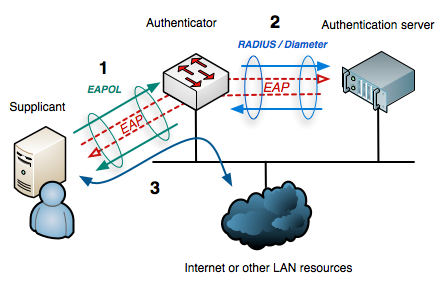
\includegraphics[scale=1]{img/auth_1x.png}
    \decoRule
    \caption{IEEE 802.1X standard architecture.}
    \label{fig:auth_1x}
\end{figure}

Supplicants use the EAP protocol\footnote{Extensible Authentication Protocol (EAP) is an authentication framework for providing the transport and usage of material and parameters generated by EAP methods.} to exchange data with the authentication server by means of the authenticator itself. EAP itself is encapsulated into other protocols; when this communication ends, the authenticator will be able to known what the supplicant is authorized to do (like accessing the Internet or certain devices/services in the LAN). The main goal is in fact understanding if the user is authorized (or not) to use available resources.
 
Even though there might be multiple authenticators, supplicants talk to just one of them at a time. The same goes for the authentication server, which is a point on which the authenticator can rely for the authentication service, but it could be made of a server federation or something like that (it is not important to the standard).

The communication channel between authenticator and server is secure, which means that the identity of the authentication server and the authenticator, between each other, is well known in advance: no attacker could sniff of inject data in this channel. Note that this level of security  can be attained by any means, as its implementation is not part of the standard. Practically speaking, we could have a VPN, a TLS channel, even have a physically secure device/network like an Ethernet cable protected by an iron cube, sharks, lasers, crocodiles, whatever. If the channel passes through unsecure areas, then it must be secured by any other means.

The channel between supplicant and authenticator is private \textit{after} authentication; even though it might not be already secured, it is not shared nonetheless, because data that passes through it (the supplicant's identity and how it is performing authentication) is critical and unprotected. Since we cannot establish an authenticated secure channel before authentication, this means that the channel between supplicant and authenticator must be secured through a generic method (even a preshared or fake authentication) in order to actually have a little bit of secrecy while the system is authenticating.

\vspace{0.5em}

\emph{Example} A Wi-Fi channel is shared until we do authentication and authorization. Vice versa, trying to authenticate to an Internet switch does not require this first phase because there is a physical connection in between (it actually depends on the context; however, the probabilities that an attacker could sniff data on a sane and untouched/well-behaving Ethernet cable are slim to none).

\vspace{0.5em}
 
%-------------------------------------------

\subsection{802.1X protocols}
The protocols that are part of the standard are two:

\begin{itemize}
	\item \textbf{EAP}: it defines how the supplicant and the authentication server exchange the material to authenticate each other; being an \textit{extensible} protocol, it does not define only one way to authenticate, but a whole class of authentication methods. By itself, EAP defines only data exchanges, while the protocols actually used to clarify the identity of the supplicant or the server are up to further specifications (there a number of different EAP flavors, some more robust than others);
	\item \textbf{EAPOL}: the way used by EAP to protect inner authenticators while they are in a shared medium; EAPOL can be skipped if we are sure that there cannot be an attacker inside the medium.
\end{itemize}

There is actually another protocol, the \textbf{RADIUS}/Diameter, although it could be replaced by any AAA protocol able to exchange EAP data between authenticator and server. This third protocol is needed because EAP only defines how the credentials are generated and how they are exchanged, but the way they are moved from the authenticator to the server is not specified. From another perspective, EAP tells us what the data is, while RADIUS/Diameter transmit the packets.

Historically speaking there have been three main AAA protocols:

\begin{itemize}
	\item \textbf{TACACS}: this one is history, not even worth mentioning;
	\item \textbf{RADIUS}: the most used one nowadays; it has been used for a long time, and it has been demonstrated to have some vulnerabilities by bad design (although they have mitigations);
	\item \textbf{Diameter}: second, better, version of RADIUS, it is far more complicated, making its acceptance questionable and hindered. Unlike RADIUS, it natively supports authentication server federations.
\end{itemize}
 
%-------------------------------------------

\subsection*{Final notes}
After authentication and authorization have been performed, there is a phase where the standard 802.1X says that, depending on the specific application, the authentication server will exchange with the supplicant and the authenticator some key material that will enable them to continue without it from there on. During this whole process the authenticator does not want and does not know (it actually never knows) who the supplicant is, but only what he/she is authorized to do.

\vspace{0.5em}

\emph{Example} Take a Wi-Fi system: the authentication server will end the authentication phase by providing the client (the supplicant) with enough information to enable it to negotiate with the authenticator some cryptographic keys without communicating them on the channel in clear text, and it will also send the same material to the authenticator. This way authenticator and supplicant will be able to go on further by themselves.

\vspace{0.5em}

Another point that is often forgotten is that the server will tell the authenticator what the client is able to do; it is not only a matter of \textit{“I found the user, here is some data to create a secure channel”}, but rather of \textit{“I found the user, here is what he/she can do on the system and here is the data”}, meaning that the authentication server is able to tell the authenticator, through RADIUS or Diameter, what are the user's setups in terms of firewall, networks, priorities of packets, use of given protocols, how much bandwidth he/she can use, etc. This is legal, and it is \textit{the} intended use of 802.1X: telling the authenticator what are the user's permissions; if we do not do this we use just $\frac{1}{3}$ of the protocol, as we are using the authentication part but forget about authorization (very much like using a cannon to kill a mosquito). Interesting enough, practically everything that implements 802.1X does exactly this. The moral of this story is that we should always learn about all the capabilities of our tools and use them accordingly.